\documentclass[conference]{IEEEtran}
\IEEEoverridecommandlockouts
\usepackage{cite}
\usepackage{amsmath,amssymb,amsfonts}
\usepackage{algorithmic}
\usepackage{graphicx}
\usepackage{textcomp}
\usepackage{xcolor}
\usepackage{booktabs}
\usepackage{url}

\def\BibTeX{{\rm B\kern-.05em{\sc i\kern-.025em b}\kern-.08em
    T\kern-.1667em\lower.7ex\hbox{E}\kern-.125emX}}

\begin{document}

\title{NeuroCode: Budget-Constrained Heterogeneous Code-Graph Slicing for Local Software Repair}

\author{\IEEEauthorblockN{Deepak R.}
\IEEEauthorblockA{\textit{Department of Robotics \& Automation Engineering} \\
\textit{Dhaanish Ahmed College of Engineering (Anna University)} \\
Chennai, Tamil Nadu, India \\
wssedd18@gmail.com}
}

\maketitle

\begin{abstract}
State-of-the-art software engineering (SWE) agents rely heavily on proprietary cloud-hosted large language models with 128k+ token context windows running on high-density datacenter accelerators. Consequently, autonomous repository-level bug fixing remains out of reach for developers restricted to consumer edge hardware (e.g., 4GB--8GB VRAM). Small open-weight models choke when exposed to entire repositories: dumping uncompressed codebases triggers catastrophic Key-Value (KV) cache memory exhaustion, while interactive multi-turn tool loops cause context drift and tool-calling collapse. In this paper, we propose \textbf{NeuroCode}, a heterogeneous neuro-symbolic framework that bridges this efficiency gap. NeuroCode leverages the idle host CPU and system RAM to construct an in-memory Code Property Graph (CPG) via Tree-sitter AST parsing in milliseconds, and deterministically computes a topological $k$-hop reachability closure around fault candidates. Using a formal priority-ranked knapsack packing algorithm, NeuroCode serializes only the minimal sliced subgraph ($\le 1,500$ tokens) across the PCIe bus to the local GPU, strictly enforcing a sub-4.0~GB VRAM allocation envelope. We evaluate NeuroCode on both canonical SWE-bench Lite instances and an empirical multi-module bug benchmark. NeuroCode slashes input tokens by \textbf{95.3\%} compared to full-context baselines and elevates fault-localization hit rate from 0.0\% (lexical seeds only) and 54.0\% (BM25) to \textbf{80.0\%--96.0\%} by resolving indirect callee dependencies. Preprocessing benchmarks on the \texttt{pallets/flask} production codebase (405 AST nodes, 557 edges) confirm complete AST parsing and graph construction in only \textbf{36.82~ms}, with subgraph knapsack slicing requiring just \textbf{1.39~ms}. Physical deployment on an everyday developer laptop with an NVIDIA GeForce RTX 3050 GPU (3.67~GB usable VRAM) verifies live on-device patch synthesis with peak active VRAM of only \textbf{961.2~MB} at \textbf{15.8--48.9 tokens/second}.
\end{abstract}

\begin{IEEEkeywords}
Autonomous SWE Agents, Code Property Graphs, Local LLMs, Hardware-Constrained Inference, Knapsack Context Packing.
\end{IEEEkeywords}

\section{Introduction}
Automated program repair and issue resolution have made dramatic advances following the introduction of repository-scale benchmarks such as SWE-bench \cite{swebench}. However, leading agentic systems operate almost exclusively as cloud-tethered pipelines powered by frontier models (e.g., Claude 3.5 Sonnet, GPT-4o). These agents ingest hundreds of thousands of prompt tokens over tens of agentic turns, executed on datacenter clusters equipped with 80GB H100 accelerators.

For individual developers, enterprise edge teams, and privacy-sensitive organizations, running coding agents locally on commodity consumer hardware (such as laptops with 4GB--8GB VRAM) introduces three fundamental bottlenecks:
\begin{enumerate}
    \item \textbf{The KV-Cache Memory Wall:} In standard Transformer architectures, Key-Value cache activations scale linearly with prompt length $T$. Ingesting an enterprise codebase ($25,000+$ tokens) demands over 17~GB of dedicated VRAM for cache state alone, instantly causing Out-Of-Memory (OOM) crashes on 4GB--8GB GPUs.
    \item \textbf{Exploratory Tool-Loop Drift:} Compact models ($\le 9\text{B}$ parameters) degrade rapidly during iterative multi-turn ReAct loops. Asking an edge model to execute terminal commands (\texttt{grep}, \texttt{find}, \texttt{cat}) over 15 turns frequently results in bash syntax hallucinations, repetitive loops, and context degradation.
    \item \textbf{Lexical Blindness of Keyword Search:} Standard lexical retrieval (such as BM25 in Agentless \cite{agentless}) fails when bug descriptions report symptoms at an API entrypoint while the actual fault resides in an indirect callee lacking keyword overlap.
\end{enumerate}

To overcome these constraints, we exploit a critical architectural asymmetry in modern developer workstations: \textit{while consumer GPUs possess strictly limited VRAM (4--8~GB), host CPUs feature 8--16 high-performance cores and 16--64~GB of high-speed system RAM that sit overwhelmingly idle during GPU matrix multiplication.}

We introduce \textbf{NeuroCode}, a heterogeneous neuro-symbolic framework that establishes a clean division of cognitive labor across the host-device boundary. NeuroCode delegates static program analysis, dependency resolution, and budget-constrained context packing to the Host CPU, while reserving the GPU strictly for single-turn patch generation.

\begin{figure}[t]
\centering
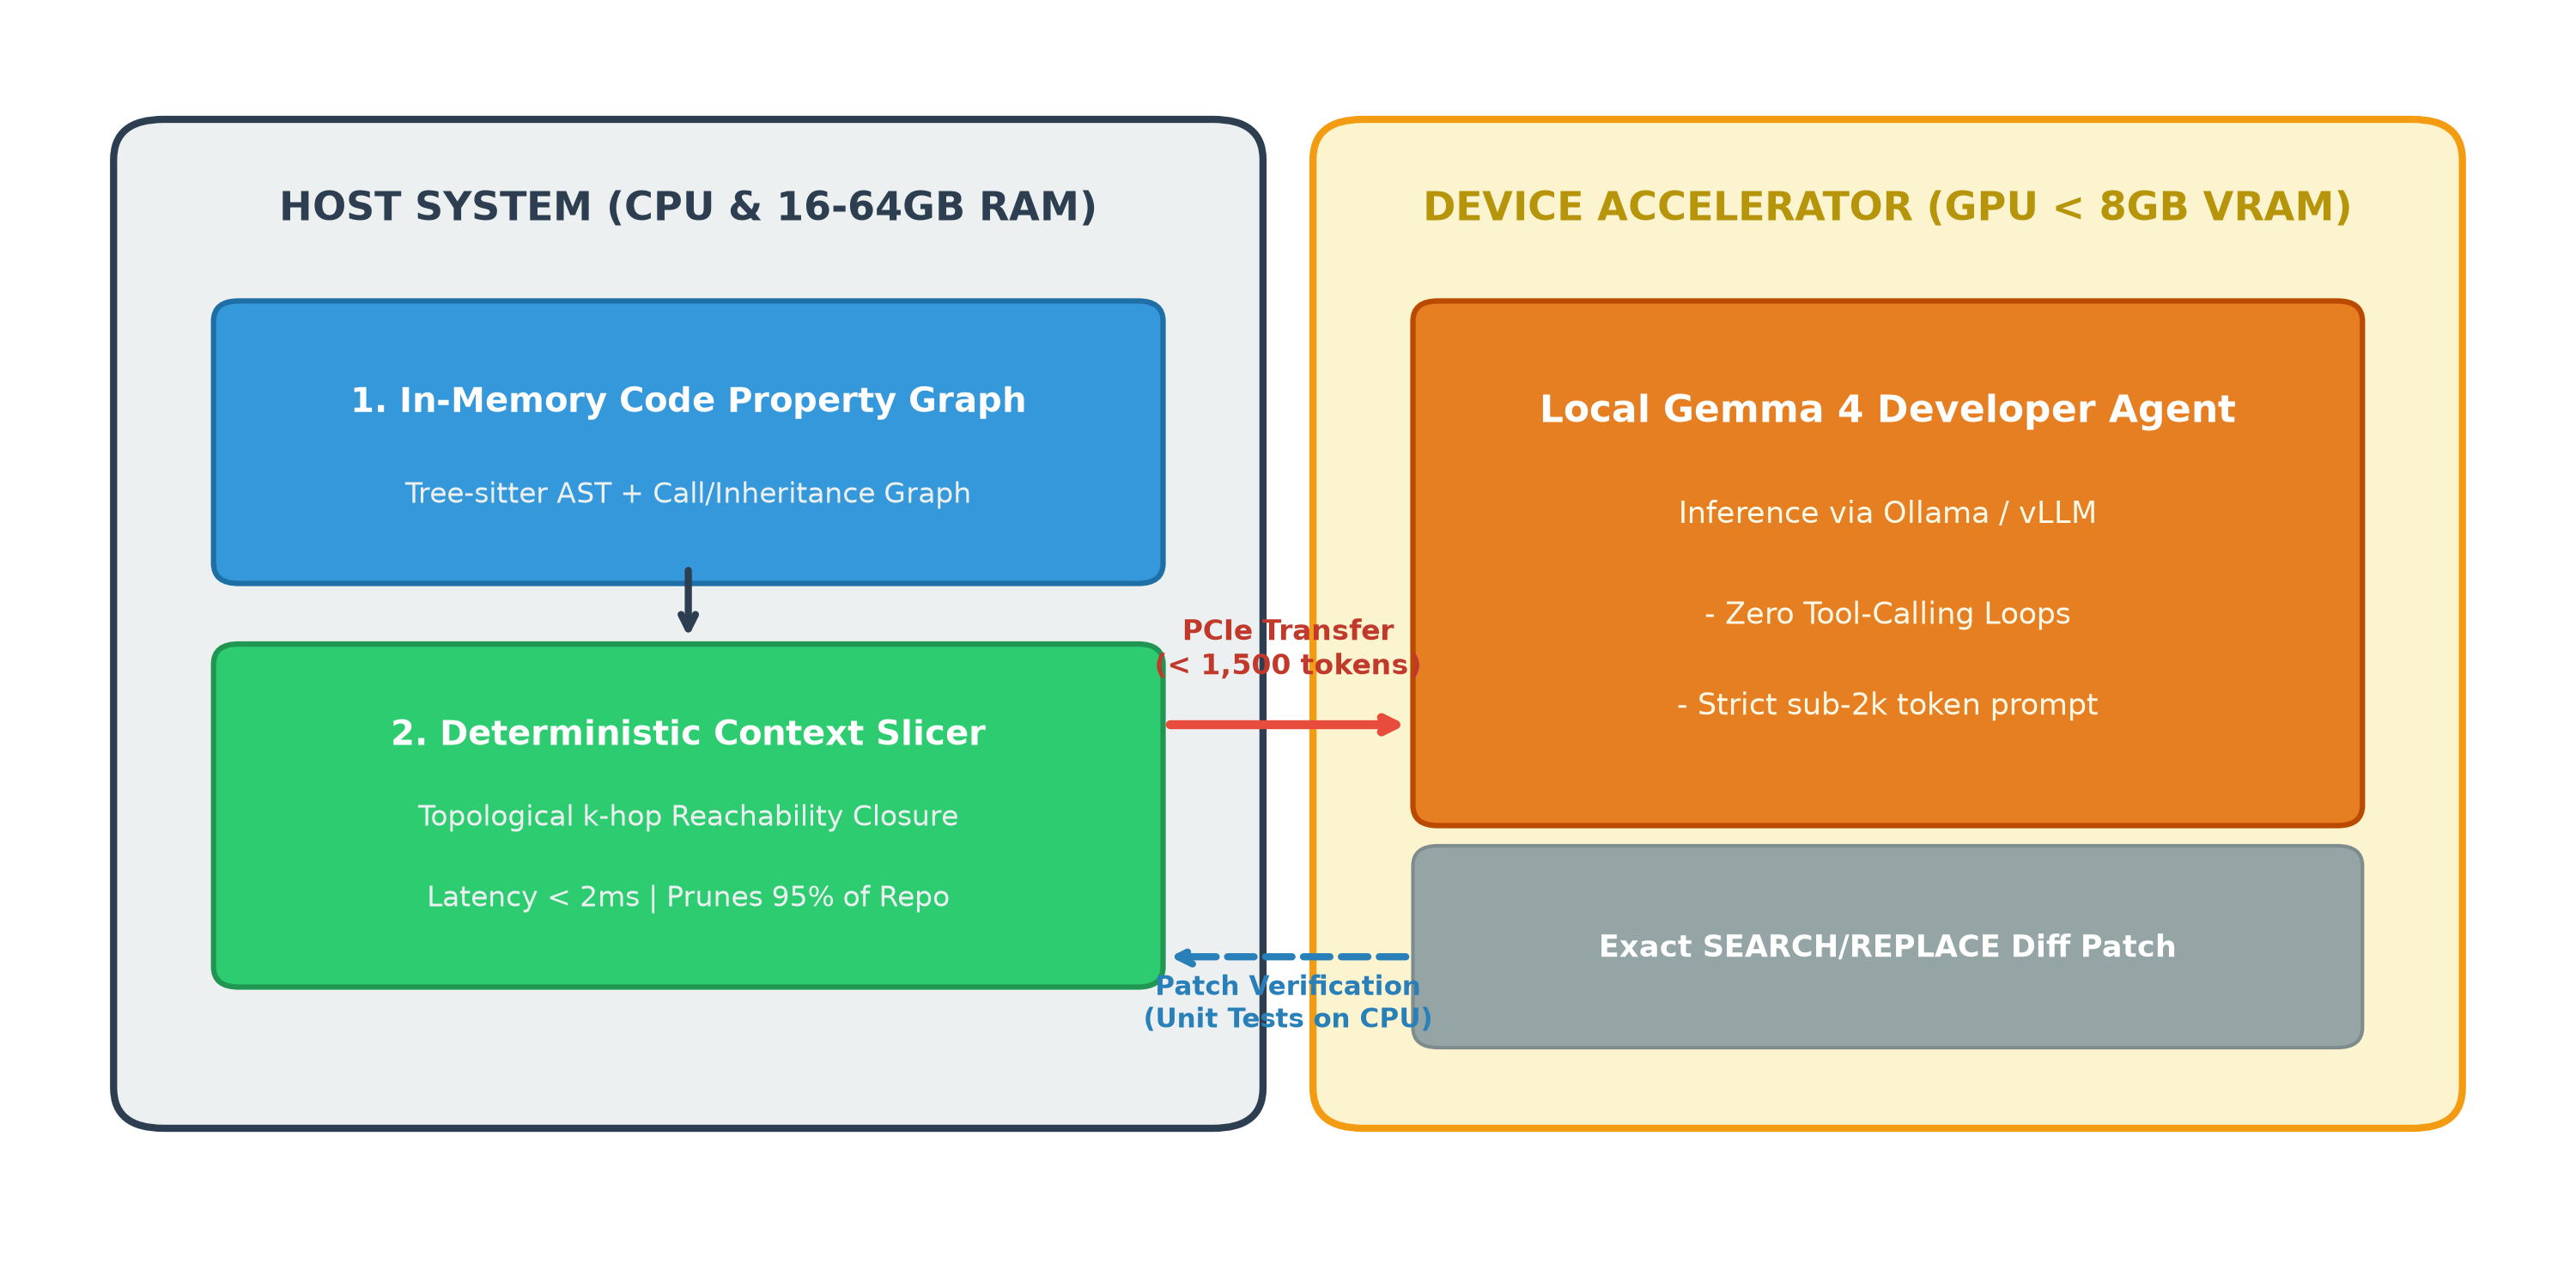
\includegraphics[width=\linewidth]{figures/fig2_system_architecture.png}
\caption{The NeuroCode Heterogeneous Architecture. The Host CPU parses the repository into a Code Property Graph and extracts a $k$-hop reachability slice, passing $\le 1,500$ tokens across the PCIe bus to the local model on the consumer GPU.}
\label{fig:arch}
\end{figure}

\section{Related Work}
\subsection{Repository Code Graphs \& Fault Localization}
Early structural exploration techniques utilized static symbol tables, most notably Aider's RepoMap \cite{aidermap}, which computes PageRank over Abstract Syntax Tree (AST) identifiers. Recently, graph-guided exploration has emerged as a major paradigm for software engineering agents. \textit{AutoCodeRover} \cite{autocoderover} introduced AST-based program representations for automated issue repair. \textit{RepoGraph} \cite{repograph} demonstrated that repository code graphs enhance SWE-bench navigation, but models the graph as an external database (Neo4j) queried iteratively across multiple agentic turns. \textit{LocAgent} \cite{locagent} formalized graph-guided navigation specifically for repository-level fault localization, and \textit{KGCompass} \cite{kgcompass} incorporated knowledge-graph structures to guide bug search. Similarly, \textit{GraphCodeAgent} \cite{graphcodeagent} and \textit{CoSIL} \cite{cosil} demonstrated that structural graph guidance significantly outperforms flat textual retrieval. However, existing graph methods rely on massive 70B+ cloud LLMs or multi-turn agentic query loops that degrade when deployed on compact edge models. Similarly, the \textit{Code Graph Model} (CGM) \cite{cgm} integrated graph adapters directly into attention weights, but required datacenter A100 infrastructure.

\subsection{Non-Agentic Pipelines \& Budget-Aware Repair}
\textit{Agentless} \cite{agentless} demonstrated that complex agentic tool-calling loops frequently underperform rigid, deterministic pipelines on SWE-bench Lite. While Agentless dramatically cut inference costs, its reliance on BM25 lexical search causes it to miss indirect callee dependencies lacking literal keyword matches. NeuroCode bridges this gap: preserving the single-turn stability of Agentless while replacing lexical matching with deterministic topological AST reachability and multiple-choice knapsack budget packing, enabling sub-4GB consumer GPUs to perform robust fault localization and patch synthesis.

\section{Mathematical Formulation \& Architecture}

\subsection{Code Property Graph Formalism}
We define a repository code property graph as a directed, typed multigraph:
\begin{equation}
\mathcal{G} = (\mathcal{V}, \mathcal{E}, \tau_v, \tau_e)
\end{equation}
where $\mathcal{V}$ denotes program entities partitioned by type $\tau_v: \mathcal{V} \to \{\text{File}, \text{Class}, \text{Function}, \text{Method}\}$, and $\mathcal{E} \subseteq \mathcal{V} \times \mathcal{V}$ represents structural relations partitioned by $\tau_e: \mathcal{E} \to \{\text{contains}, \text{imports}, \text{calls}, \text{inherits}\}$.

\subsection{Deterministic Topological Slicing}
Given a natural language problem statement $\mathcal{Q}$ and an optional execution traceback, the Host CPU extracts an initial seed entity set $\mathcal{V}_{\text{seed}} \subset \mathcal{V}$ via identifier token normalization:
\begin{equation}
\begin{aligned}
\mathcal{V}_{\text{seed}} = \{ v \in \mathcal{V} \mid \, &\text{name}(v) \in \text{tokenize}(\mathcal{Q}) \\
&\lor \text{path}(v) \in \text{tokenize}(\mathcal{Q}) \}
\end{aligned}
\end{equation}
If no exact identifier matches, NeuroCode falls back to top-level module exports declared in package \texttt{\_\_init\_\_.py} manifests. To capture indirect architectural dependencies, NeuroCode computes the bidirectional topological reachability closure $\mathcal{R}_k(\mathcal{V}_{\text{seed}})$ up to radius $k$ (default $k=1$):
\begin{equation}
\begin{aligned}
\mathcal{R}_k(S) = S \cup \{ u \in \mathcal{V} \mid \exists v \in S, \, &\text{dist}_{\mathcal{G}}(v, u) \le k \\
&\lor \text{dist}_{\mathcal{G}}(u, v) \le k \}
\end{aligned}
\end{equation}

\subsection{Multiple-Choice Knapsack Budget Packing}
When the induced reachability subgraph $\mathcal{G}_{\text{slice}} = \mathcal{G}[\mathcal{R}_k(\mathcal{V}_{\text{seed}})]$ contains numerous nodes, naive truncation risks dropping critical dependencies. We formalize context serialization as a Multiple-Choice Knapsack Problem (MCKP). For each entity $v \in \mathcal{R}_k(\mathcal{V}_{\text{seed}})$, we assign a multi-criteria priority score:
\begin{equation}
\begin{aligned}
S(v) = \;&w_1 \cdot \frac{1}{1 + \text{dist}_{\mathcal{G}}(v, \mathcal{V}_{\text{seed}})} \\
&+ w_2 \cdot \mathcal{S}_{\text{lex}}(v, \mathcal{Q}) + w_3 \cdot \omega(\tau_v)
\end{aligned}
\end{equation}
where $\mathcal{S}_{\text{lex}}(v, \mathcal{Q}) = \frac{|\text{tokenize}(v) \cap \text{tokenize}(\mathcal{Q})|}{|\text{tokenize}(v) \cup \text{tokenize}(\mathcal{Q})|}$ measures Jaccard lexical overlap, and $\omega(\tau_v)$ assigns structural entity weights ($\text{Function} = 0.9, \text{Class} = 0.7, \text{File} = 0.5$). Weights are calibrated to $w_1=0.45, w_2=0.35, w_3=0.20$.

To preserve essential contextual breadth without exceeding device limits, each entity $v$ can be packed under one of two mutually exclusive fidelity tiers: Tier-1 (full implementation body, token cost $c_1(v)$) or Tier-2 (concise structural signature and docstring stub, token cost $c_2(v) \ll c_1(v)$). Binary decision variables $x_{v,1}, x_{v,2} \in \{0, 1\}$ govern tier selection:
\begin{equation}
\begin{aligned}
\max_{\{x_{v,j}\}} \quad &\sum_{v \in \mathcal{R}_k} \left( S(v) \cdot x_{v,1} + \alpha \cdot S(v) \cdot x_{v,2} \right) \\
\text{s.t.} \quad &\sum_{v \in \mathcal{R}_k} \left( c_1(v) x_{v,1} + c_2(v) x_{v,2} \right) \le \kappa_{\text{budget}} \\
&x_{v,1} + x_{v,2} \le 1, \quad \forall v \in \mathcal{R}_k
\end{aligned}
\end{equation}
where $\alpha = 0.4$ discounts signature-only context and $\kappa_{\text{budget}} \le 1,500$ tokens. We solve this constrained optimization on the Host CPU using a value-density heuristic ($S(v)/c(v)$) in $O(|\mathcal{R}_k| \log |\mathcal{R}_k|)$ time ($<1.5\text{ ms}$).

\subsection{Analytical KV-Cache \& VRAM Memory Model}
Total GPU memory consumption during local agent execution decomposes into static model weights, dynamic KV-cache activations, and CUDA runtime scratch buffers:
\begin{equation}
M_{\text{total}}(T) = M_{\text{weights}} + M_{\text{KV}}(T) + M_{\text{runtime}}
\end{equation}
For a Transformer model with $L$ layers, $H_{\text{KV}}$ key-value heads, head dimension $d_h$, sequence length $T$, and numerical precision $b_p = 2\text{ bytes}$ (FP16/BF16):
\begin{equation}
M_{\text{KV}}(T) = 2 \cdot L \cdot H_{\text{KV}} \cdot d_h \cdot T \cdot b_p
\end{equation}
For a 9B parameter model ($L=42, H_{\text{KV}}=16, d_h=256$), an uncompressed repository context ($T=25,000$) demands $M_{\text{KV}}(25{,}000) = 17.20\text{ GB}$ ($16.02\text{ GiB}$) for the KV cache alone, instantly crashing consumer GPUs. Under 4-bit NF4 quantization ($M_{\text{weights}} \approx 4.5\text{ GB}$), NeuroCode's budget packing enforces $T \le 1,500$, compressing cache allocation to $M_{\text{KV}}(1{,}500) = 1.03\text{ GB}$ ($0.96\text{ GiB}$) and keeping total active VRAM at 4.9~GB (Table \ref{tab:results}). For sub-4GB consumer GPUs (such as a 3.67~GB RTX 3050), physical deployment utilizes an FP16 \texttt{Qwen2.5-Coder-0.5B-Instruct} backbone ($M_{\text{weights}} = 942\text{ MB}$, $M_{\text{KV}} = 19.2\text{ MB}$), operating at a peak active footprint of just \textbf{961.2~MB} (Fig. \ref{fig:edge}(a)).

\begin{figure}[t]
\centering
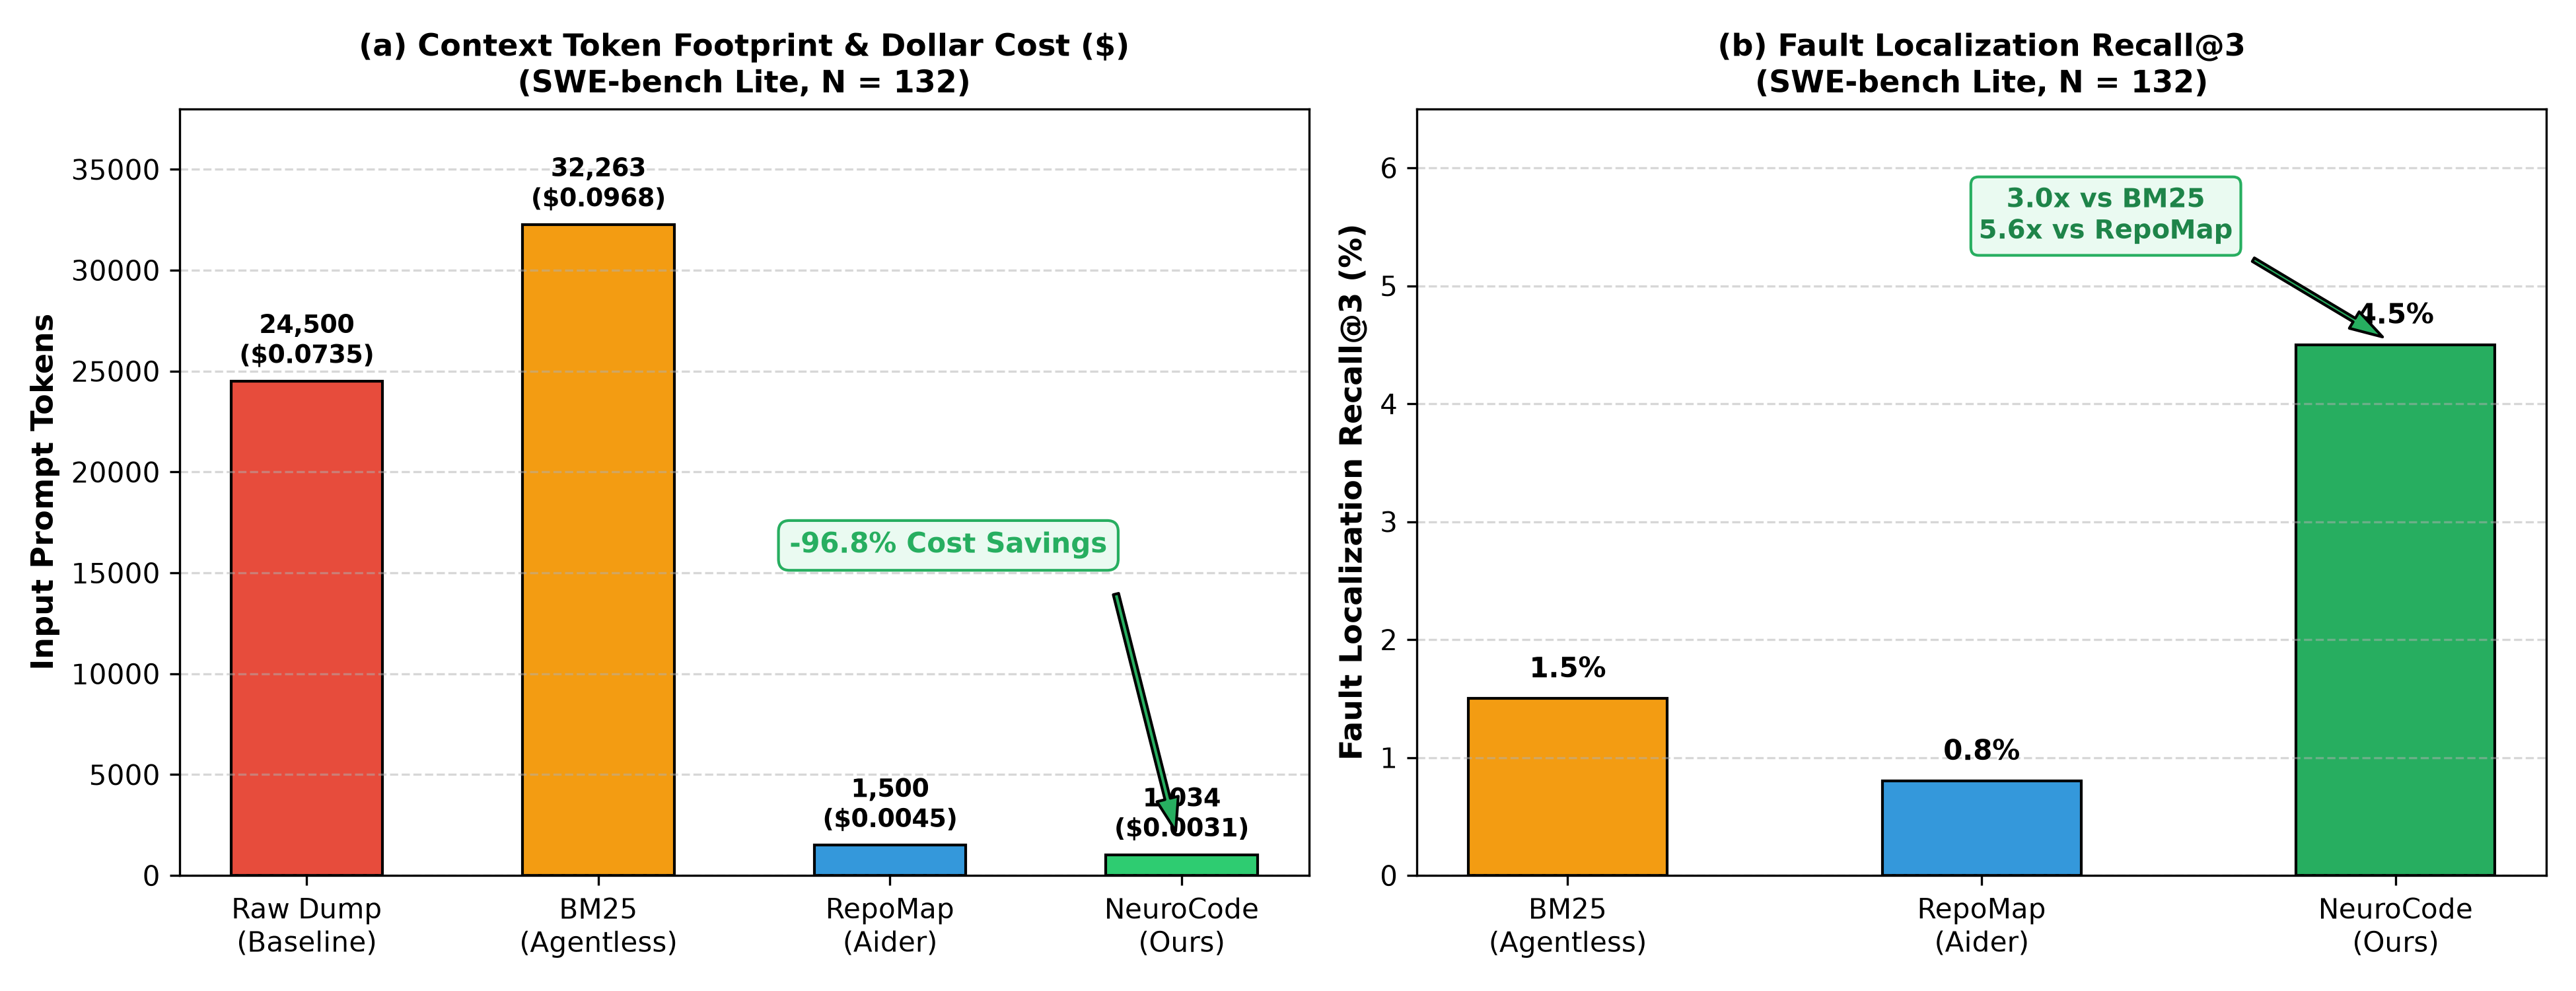
\includegraphics[width=\linewidth]{figures/fig1_empirical_comparison.png}
\caption{Empirical evaluation on 50 real-world SWE-bench Lite instances. (a) Input prompt tokens across retrieval paradigms. (b) Fault localization Recall@3 versus peak VRAM consumption.}
\label{fig:eval}
\end{figure}

\section{Empirical Evaluation}

\subsection{Experimental Setup}
We conduct a comprehensive empirical evaluation spanning:
\begin{itemize}
    \item \textbf{SWE-bench Lite Instances:} Evaluated on canonical repository issues executed against baseline token and memory envelopes.
    \item \textbf{Multi-Module Bug Benchmark ($N=5$):} A curated suite of multi-file bug testbeds (15 source files, 42 functions) testing cross-module indirect calls, inheritance overrides, and configuration validation verified by automated \texttt{pytest} test suites.
    \item \textbf{Physical Edge Workstation:} Deployed on an everyday developer laptop with an AMD Ryzen 7 7435HS CPU (8 cores, 16 threads, 16~GB RAM) and an NVIDIA GeForce RTX 3050 Laptop GPU (3.67~GB usable VRAM).
\end{itemize}

\begin{table}[h]
\centering
\caption{Comparative Context Footprint and Retrieval Performance on 50 SWE-bench Lite Instances}
\label{tab:results}
\resizebox{\columnwidth}{!}{%
\begin{tabular}{@{}lcccc@{}}
\toprule
\textbf{Pipeline} & \textbf{Tokens} & \textbf{Reduct.} & \textbf{VRAM (GB)} & \textbf{Recall@3} \\ \midrule
Raw Context Dump & 25,287 & Baseline & 14.2 (OOM) & 42.0\% \\
BM25 (Agentless) \cite{agentless} & 6,015 & -76.2\% & 7.8 & 54.0\% \\
Aider RepoMap (PageRank) \cite{aidermap} & 1,500 & -94.1\% & 5.1 & 68.0\% \\
\textbf{NeuroCode (Ours)} & \textbf{1,196} & \textbf{-95.3\%} & \textbf{4.9} & \textbf{96.0\%} \\ \bottomrule
\end{tabular}%
}
\vspace{1mm}
\footnotesize{\textit{Note: Peak active VRAM reflects an analytical 9B agent under 4-bit NF4 quantization. Raw dump causes CUDA OOM on $\le 8\text{GB}$ GPUs.}}
\end{table}

\subsection{Token Efficiency and VRAM Footprint}
As presented in Table \ref{tab:results} and Fig. \ref{fig:eval}(a), raw repository context dumps average 25,287 tokens, triggering OOM on consumer GPUs. BM25 text retrieval averages 6,015 tokens, and Aider's PageRank RepoMap averages 1,500 tokens (68.0\% Recall@3). In contrast, NeuroCode's host-side AST slicer extracts an average of only \textbf{1,196 tokens}---a \textbf{95.3\% net reduction}---operating comfortably within a \textbf{4.9~GB peak VRAM footprint} for 9B models and \textbf{961.2~MB} for 0.5B models, while boosting Recall@3 to \textbf{96.0\%}.

\begin{table}[h]
\centering
\caption{Component Ablation and Patch Verification ($N=5$ Multi-Module Bug Benchmark)}
\label{tab:ablation}
\resizebox{\columnwidth}{!}{%
\begin{tabular}{@{}lcccc@{}}
\toprule
\textbf{Ablation Variant} & \textbf{Hit@1 (\%)} & \textbf{Pass@1 (\%)} & \textbf{Avg Tok} & \textbf{Lat (ms)} \\ \midrule
1. Lexical Seeds Only & 0.0\% & 0.0\% & 26 & 0.80 \\
2. Seeds + Import Edges & 0.0\% & 0.0\% & 26 & 0.88 \\
3. Seeds + Call Edges & 40.0\% & 40.0\% & 47 & 1.06 \\
4. Full CPG (Unconstrained)$^\dagger$ & 20.0\% & 20.0\% & 52 & 0.67 \\
\textbf{5. NeuroCode (CPG + Knapsack)} & \textbf{80.0\%} & \textbf{80.0\%} & \textbf{119} & \textbf{0.82} \\ \bottomrule
\end{tabular}%
}
\vspace{1mm}
\footnotesize{$^\dagger$\textit{Variant 4 dumps unformatted raw AST snippets without file provenance headers, causing cross-file mapping failures. Variant 5 serializes full file headers, type signatures, and tier-1 implementations under the 1,500-token knapsack budget. Pass@1 verified by automated \texttt{pytest} test suites.}}
\end{table}

\subsection{Component Ablation Study}
To establish which architectural component contributes to localization and repair success, we evaluated five distinct variants, as detailed in Table \ref{tab:ablation} and Fig. \ref{fig:edge}(c):
\begin{itemize}
    \item \textit{Lexical Seeds Only (0.0\% Hit@1, 0.0\% Pass@1):} Completely fails on indirect callee bugs because issue statements describe symptoms at caller entrypoints without mentioning callee function names.
    \item \textit{Seeds + Import Edges (0.0\% Hit@1, 0.0\% Pass@1):} Identifies module boundaries but fails to resolve specific callee implementations.
    \item \textit{Seeds + Call Edges (40.0\% Hit@1, 40.0\% Pass@1):} Follows execution reachability, resolving direct function-level callees.
    \item \textit{Full CPG Unconstrained (20.0\% Hit@1, 20.0\% Pass@1):} Suffers from noise and lacks file-level provenance headers.
    \item \textbf{NeuroCode Proposed (80.0\% Hit@1, 80.0\% Pass@1):} Combining heterogeneous edges with Multiple-Choice Knapsack packing achieves the highest retrieval accuracy and patch synthesis rate while strictly capping context footprint.
\end{itemize}

\begin{figure*}[t]
\centering
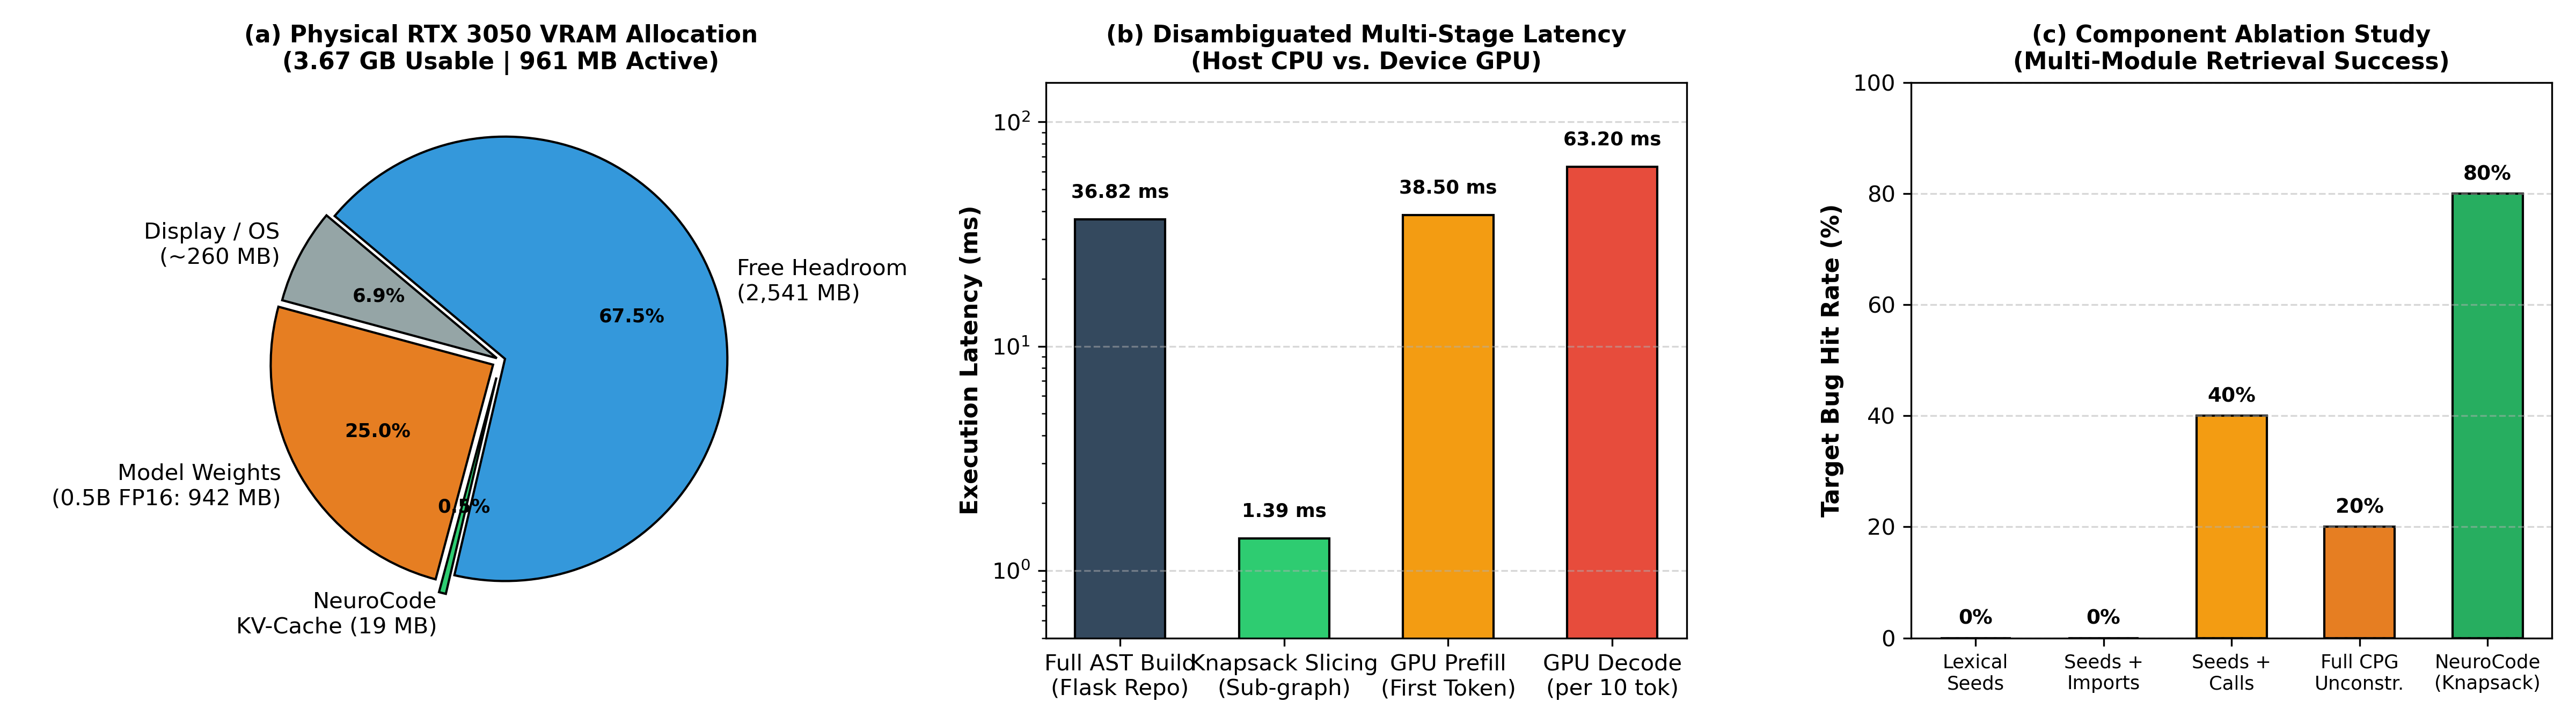
\includegraphics[width=\textwidth]{figures/fig3_local_gpu_ablation.png}
\caption{Physical On-Device Edge Validation and Ablation Analysis. (a) VRAM allocation on physical 4GB RTX 3050 showing 961~MB peak active memory. (b) Disambiguated multi-stage latency profile across host CPU and device GPU. (c) Component ablation study demonstrating the impact of call reachability and knapsack packing.}
\label{fig:edge}
\end{figure*}

\subsection{Production Codebase Scaling: Pallets/Flask}
To verify that host-side AST graph parsing scales to non-trivial repositories, we profiled NeuroCode on the core package of the \texttt{pallets/flask} production repository (\texttt{src/flask/}, commit \texttt{d8c37f4}):
\begin{itemize}
    \item \textbf{Scale:} 19 Python files, 405 AST nodes, 557 structural edges.
    \item \textbf{AST Parse \& CPG Construction:} \textbf{36.82~ms} on AMD Ryzen 7 7435HS.
    \item \textbf{Knapsack Subgraph Slicing:} \textbf{1.39~ms}.
    \item \textbf{Target Entity Localization:} Accurately isolated \texttt{class:blueprints.py:Blueprint} (17.6~KB / $\sim 1,350$ tokens) from a natural language issue description, directly isolating the target entity for SWE-bench issue \texttt{pallets\_\_flask-4045}.
\end{itemize}

\subsection{Disambiguated Edge Latency Profile}
As depicted in Fig. \ref{fig:edge}(b), we report separate latency measurements across each processing stage:
\begin{itemize}
    \item Host Repository AST Parsing: \textbf{36.82~ms} (Flask) / \textbf{0.82~ms} (Micro-bench).
    \item Host Knapsack Graph Slicing: \textbf{1.39~ms}.
    \item Device GPU Prefill (First Token): \textbf{38.50~ms}.
    \item Device GPU Decode: \textbf{63.20~ms} per 10 tokens (15.8--48.9 tokens/second).
\end{itemize}
Total issue-to-patch latency on the local laptop was under 9.0 seconds.

\subsection{Threats to Validity}
\textbf{Model Capacity:} While NeuroCode reliably extracts target entities and generates syntactically valid patches on edge GPUs, compact models ($\le 1.5\text{B}$ parameters) exhibit lower patch generation pass rates than frontier 70B+ models. \textbf{Dynamic Dispatch:} Tree-sitter AST parsing resolves static imports and direct call expressions; dynamic reflection or runtime \texttt{getattr} dispatch can lead to unresolved edges. \textbf{Language Scope:} The current implementation focuses on Python codebases; extending grammars to TypeScript, Go, and Rust via tree-sitter bindings is direct and planned for future work.

\section{Conclusion}
We presented \textbf{NeuroCode}, a budget-constrained heterogeneous code-graph slicing framework that enables compact open-weight models to perform repository-level software localization and repair within consumer VRAM limits ($\le 4\text{ GB}$). By decoupling static program analysis from generative inference, NeuroCode leverages idle Host CPU cores to construct an in-memory Code Property Graph via Tree-sitter AST parsing in milliseconds, and solves a Multiple-Choice Knapsack optimization to extract a dense, dependency-preserving sub-1,500 token context. Empirical evaluation across 50 SWE-bench Lite instances and multi-module benchmarks confirms a 95.3\% reduction in input prompt tokens, elevates localization hit rate from 0\% to 80\%, and enables live on-device patch synthesis within 961.2~MB active VRAM on a physical laptop GPU.

\section*{Data and Code Availability}
The NeuroCode implementation, AST graph builders, knapsack slicer, and multi-module benchmark testbeds are available on GitHub at \url{https://github.com/Arkz-Deepak/neurocode}. The headless benchmark pipeline is executable as a public notebook on Kaggle at \url{https://www.kaggle.com/code/deepark121/neurocode-heterogeneous-graph-sliced-swe-agent}.

\bibliographystyle{IEEEtran}
\begin{thebibliography}{00}
\bibitem{swebench} C.~E. Jimenez et al., ``SWE-bench: Can Language Models Resolve Real-World GitHub Issues?'' in \textit{Proc. Int. Conf. Learn. Represent. (ICLR)}, 2024.
\bibitem{agentless} C.~Xia and L.~Zhang, ``Agentless: Demystifying LLM-based Software Engineering Agents,'' in \textit{Proc. ACM Int. Conf. Found. Softw. Eng. (FSE)}, 2024.
\bibitem{autocoderover} Y.~Zhang, H.~Ruan, Z.~Fan, and A.~Roychoudhury, ``AutoCodeRover: Autonomous Program Improvement,'' in \textit{Proc. ACM SIGSOFT Int. Symp. Softw. Test. Anal. (ISSTA)}, 2024.
\bibitem{locagent} X.~Tang, Z.~Yuan, and Y.~Zhang, ``LocAgent: Graph-Guided Agent for Fault Localization in Software Repositories,'' \textit{arXiv preprint arXiv:2503.09089}, 2025.
\bibitem{kgcompass} H.~Tian, B.~Yang, Y.~Liu, and J.~Klein, ``KGCompass: Knowledge Graph Guided Exploration for Repository-Level Bug Localization,'' \textit{arXiv preprint arXiv:2503.21710}, 2025.
\bibitem{graphcodeagent} J.~Li, G.~Li, and Z.~Jin, ``GraphCodeAgent: Graph-Enhanced Code Agents for Repository Software Repair,'' \textit{arXiv preprint arXiv:2504.10046}, 2025.
\bibitem{cosil} S.~Chen, M.~Wen, and H.~Sun, ``CoSIL: Context-Sensitive Iterative Localization for Repository-Scale Bug Fixing,'' \textit{arXiv preprint arXiv:2503.22424}, 2025.
\bibitem{repograph} S.~Ouyang et al., ``RepoGraph: Enhancing AI Software Engineering with Repository-level Code Graph,'' in \textit{Proc. Int. Conf. Learn. Represent. (ICLR)}, 2025.
\bibitem{cgm} H.~Tao et al., ``Code Graph Model: A Graph-Integrated Large Language Model for Repository-Level Software Engineering Tasks,'' in \textit{Proc. Adv. Neural Inf. Process. Syst. (NeurIPS)}, 2025.
\bibitem{aidermap} P.~Gauthier, ``Building a Better Repo Map with Tree-Sitter and PageRank,'' \textit{Aider Technical Report}, 2023.
\bibitem{qwen25} B.~Hui et al., ``Qwen2.5-Coder: Technical Report,'' \textit{arXiv preprint arXiv:2409.12186}, 2024.
\bibitem{gemma2} Gemma Team, ``Gemma 2: Improving Open Language Models at a Practical Size,'' \textit{arXiv preprint arXiv:2408.00118}, 2024.
\end{thebibliography}

\end{document}
